\documentclass[12pt,a4paper]{article}
\def\ntitle{Algebraic Topology}

% --- Core Mathematical Packages ---
\usepackage{amsmath}
\usepackage{amssymb}
\usepackage{amsthm}
\usepackage{bm}

% --- Page Layout & Headers ---
\usepackage{geometry}
\geometry{
    a4paper,
    margin=1in,
    headheight=15pt
}
\usepackage{fancyhdr}
\pagestyle{fancy}
\fancyhf{}
\fancyfoot[C]{\thepage}
\lhead{\emph{\nouppercase{\leftmark}}}

% --- Typography, Lists & Helpers ---
\usepackage{enumitem}
\usepackage{etoolbox}
\usepackage{caption}
\usepackage{pgffor}
\usepackage{xcolor}
\usepackage{tikz}
\usetikzlibrary{arrows.meta, positioning}

% List formatting
\renewcommand{\theenumi}{\alph{enumi}}
\renewcommand{\labelenumi}{(\theenumi)}
\setlist[itemize,2]{label=$\circ$}
\setlist{
    topsep=3pt,
    itemsep=2pt,
    parsep=0pt,
    before=\leavevmode
}

% Paragraph layout: zero indentation, clean inter-paragraph glue
\setlength{\parindent}{0pt}
\setlength{\parskip}{5pt plus 2pt minus 1pt}

% Document Metadata
\author{ioshift}
\date{\today}
\title{\Huge\bfseries\ntitle}


%%%%%%%%%%%%%%%%%%%%%%%%%%%%%%%%%%%%%%%%%%%%%%%%%%%%%%%%%%%%%%%%%%%%%%%%%%%%%%%
%% Theorem Environments & Styling
%%%%%%%%%%%%%%%%%%%%%%%%%%%%%%%%%%%%%%%%%%%%%%%%%%%%%%%%%%%%%%%%%%%%%%%%%%%%%%%

\numberwithin{equation}{subsection}

% Custom Theorem Styles with built-in vertical glue
\newtheoremstyle{notestyle_thm}
  {6pt plus 2pt minus 1pt}  % Space above
  {6pt plus 2pt minus 1pt}  % Space below
  {\normalfont}             % Body font
  {}                        % Indent amount
  {\bfseries}               % Head font
  {.}                       % Punctuation after head
  { }                       % Space after head
  {}                        % Head spec

\newtheoremstyle{notestyle_remark}
  {5pt plus 2pt minus 1pt}  % Space above
  {5pt plus 2pt minus 1pt}  % Space below
  {\normalfont}             % Body font
  {}                        % Indent amount
  {\bfseries}               % Head font
  {.}                       % Punctuation after head
  { }                       % Space after head
  {}                        % Head spec

% Numbered theorem-like environments
\theoremstyle{notestyle_thm}
\newtheorem{thm}{Theorem}[subsection]
\renewcommand{\thethm}{%
  \ifnum\value{subsection}=0
    \thesection.\arabic{thm}%
  \else
    \thesubsection.\arabic{thm}%
  \fi
}

\newtheorem{axiom}[thm]{Axiom}
\newtheorem{conjecture}[thm]{Conjecture}
\newtheorem{cor}[thm]{Corollary}
\newtheorem{eg}[thm]{Example}
\newtheorem{prop}[thm]{Proposition}
\newtheorem{lemma}[thm]{Lemma}
\newtheorem{ex}[thm]{Exercise}
\newtheorem{definition}[thm]{Definition}
\newtheorem{notations}[thm]{Notation}

% Unnumbered / Starred environments
\theoremstyle{notestyle_remark}
\newtheorem*{aim}{Aim}
\newtheorem*{assumption}{Assumption}
\newtheorem*{claim}{Claim}
\newtheorem*{Defi}{Definition}
\newtheorem*{fact}{Fact}
\newtheorem*{law}{Law}
\newtheorem*{remark}{Remark}
\newtheorem*{note}{Note}
\newtheorem*{rrule}{Rule}
\newtheorem*{Prop}{Proposition}
\newtheorem*{question}{Question}
\newtheorem*{warning}{Warning}

% Proof & Solution Environments
\renewcommand{\proofname}{\textbf{Proof}}
\newenvironment{sol}{\begin{proof}[\textbf{Solution}]}{\end{proof}}
\newenvironment{counter}{\begin{proof}[\textbf{Counterexample}]}{\end{proof}}


%%%%%%%%%%%%%%%%%%%%%%%%%%%%%%%%%%%%%%%%%%%%%%%%%%%%%%%%%%%%%%%%%%%%%%%%%%%%%%%
%% Mathematical Macros & Symbols
%%%%%%%%%%%%%%%%%%%%%%%%%%%%%%%%%%%%%%%%%%%%%%%%%%%%%%%%%%%%%%%%%%%%%%%%%%%%%%%

% Standard blackboard-bold sets
\newcommand{\C}{\mathbb{C}}
\newcommand{\R}{\mathbb{R}}
\newcommand{\Q}{\mathbb{Q}}
\newcommand{\Z}{\mathbb{Z}}
\newcommand{\N}{\mathbb{N}}
\newcommand{\F}{\mathbb{F}}

% Calligraphic collections
\newcommand{\topo}{\mathcal{T}}

% Mathematical Operators
\DeclareMathOperator{\re}{Re}
\DeclareMathOperator{\im}{Im}
\DeclareMathOperator{\interior}{Int}
\DeclareMathOperator{\lcm}{lcm}
\DeclareMathOperator{\diam}{diam}
\DeclareMathOperator{\id}{id}
\DeclareMathOperator{\Bd}{Bd}
\DeclareMathOperator{\card}{card}
\DeclareMathOperator{\supp}{supp}
\DeclareMathOperator{\image}{im}

% Delimiters & Accents
\newcommand{\abs}[1]{\left\lvert #1 \right\rvert}
\newcommand{\norm}[1]{\left\lVert #1 \right\rVert}
\newcommand{\floor}[1]{\left\lfloor #1 \right\rfloor}
\newcommand{\ceil}[1]{\left\lceil #1 \right\rceil}
\newcommand{\set}[1]{\left\{ #1 \right\}}
\newcommand{\closure}[2][3]{{}\mkern#1mu\overline{\mkern-#1mu#2}}
\newcommand{\group}[1]{\langle #1 \rangle}

% Symbols & Relations
\newcommand{\noteq}{\neq}
\newcommand{\nexist}{\nexists}
\newcommand{\aand}{\quad\text{and}\quad}
\newcommand{\res}[1]{\!\mid_{#1}}
\newcommand{\normal}{\unlhd}
\renewcommand{\tt}[1]{\quad\text{#1}\quad}
\renewcommand{\d}{\mathop{}\!\mathrm{d}}
\renewcommand{\emptyset}{\varnothing}

% Darboux / Riemann integrals
\newcommand{\upint}{\mathchoice%
    {\mkern13mu\overline{\vphantom{\intop}\mkern7mu}\mkern-20mu}%
    {\mkern7mu\overline{\vphantom{\intop}\mkern7mu}\mkern-14mu}%
    {\mkern7mu\overline{\vphantom{\intop}\mkern7mu}\mkern-14mu}%
    {\mkern7mu\overline{\vphantom{\intop}\mkern7mu}\mkern-14mu}%
  \int}
\newcommand{\lowint}{\mkern3mu\underline{\vphantom{\intop}\mkern7mu}\mkern-10mu\int}


%%%%%%%%%%%%%%%%%%%%%%%%%%%%%%%%%%%%%%%%%%%%%%%%%%%%%%%%%%%%%%%%%%%%%%%%%%%%%%%
%% Automatic Definition & Concept Glossary Engine
%%%%%%%%%%%%%%%%%%%%%%%%%%%%%%%%%%%%%%%%%%%%%%%%%%%%%%%%%%%%%%%%%%%%%%%%%%%%%%%

\newcounter{cnt}

\newcommand{\newterm}[3]{%
    \expandafter\gdef\csname term#1\endcsname{#2}%
    \expandafter\gdef\csname cat#1\endcsname{#3}%
}

% Definition environment with automatic glossary registration
\newenvironment{defi}[1]{%
    \refstepcounter{cnt}%
    \phantomsection\label{glo:\arabic{cnt}}%
    \newterm{\arabic{cnt}}{#1}{0}%
    \begin{definition}\textbf{#1}
    
}{%
    \end{definition}%
}

% Notation environment with automatic glossary registration
\newenvironment{notation}[1]{%
    \refstepcounter{cnt}%
    \phantomsection\label{glo:\arabic{cnt}}%
    \newterm{\arabic{cnt}}{#1}{0}%
    \begin{notations}\textbf{#1}
    
}{%
    \end{notations}%
}

% Ad-hoc glossary elements and category headers
\newcommand{\addelement}[1]{%
    \refstepcounter{cnt}%
    \phantomsection\label{glo:\arabic{cnt}}%
    \newterm{\arabic{cnt}}{#1}{0}%
}

\newcommand{\addclass}[1]{%
    \refstepcounter{cnt}%
    \phantomsection\label{glo:\arabic{cnt}}%
    \newterm{\arabic{cnt}}{#1}{1}%
}

% Glossary rendering command
\newcommand{\printglossary}{%
    \newpage
    \section{Glossary}
    \ifnum\value{cnt}>0
      \foreach \x in {1,...,\arabic{cnt}} {%
          \ifnum\csname cat\x\endcsname=0
              \noindent\hyperref[glo:\x]{\csname term\x\endcsname}\par\addvspace{0.4em}%
          \else
              \ifnum\x>1
                  \addvspace{1.2em}%
              \fi
              \noindent{\large\textbf{\csname term\x\endcsname}}\par\addvspace{0.6em}%
          \fi
      }%
    \fi
}


%%%%%%%%%%%%%%%%%%%%%%%%%%%%%%%%%%%%%%%%%%%%%%%%%%%%%%%%%%%%%%%%%%%%%%%%%%%%%%%
%% Hyperref (Loaded Last for Guaranteed Compatibility)
%%%%%%%%%%%%%%%%%%%%%%%%%%%%%%%%%%%%%%%%%%%%%%%%%%%%%%%%%%%%%%%%%%%%%%%%%%%%%%%

\usepackage[colorlinks=true, linkcolor=red, citecolor=red, urlcolor=blue]{hyperref}

\begin{document}

    % --- Front Matter ---
    \pagenumbering{Roman}
    \maketitle
    \newpage
    \tableofcontents    
    \newpage
    \pagenumbering{arabic}

    % --- Main Document ---

    \setcounter{section}{-1}
    \section{Abstract Algebra Prerequisites}\addclass{Abstract Algebra Prerequisites}
    \subsection{Group Theory Basics}
    
    \begin{defi}{Group}
        A \textbf{group} $\group{G,*}$ is a set $G$, closed under a binary operaton $*$, which satisfies 
        \begin{itemize}
            \item associativity of $*$
            \item existence of identity element $e$
            \item existence of inverse element $a'$ of $a$ for all $a\in G$ 
        \end{itemize}
    \end{defi}
    \bigskip

    \begin{defi}{Homomorphism and Isomorphism}
        Let $\group{G_1,*_1}$ and $\group{G_2,*_2}$ be groups and $f:G_1\to G_2$. We say that $f$ is a \textbf{group isomorphism} if
        \begin{itemize}
            \item $f$ is bijective.
            \item For all $a,b\in G$, $f(a*_1b)=f(a)*_2f(b)$.
        \end{itemize}
        $f$ is a \textbf{group homomorphism} if the second condition is satisfied.
    \end{defi}
    \bigskip
    
    \begin{defi}{Permutation and Symmetric Group}
        Let $A \noteq \emptyset$. A \textbf{permutation} of $A$ is a bijection $\sigma \colon A \to A$. The \textbf{symmetric group} on $A$ is
        \[
            S_A = \operatorname{Sym}(A) = \set{\sigma \colon A \to A \mid \sigma \text{ is bijective}}
        \]
        For $A = \set{1, 2, \ldots, n}$, denote $S_n = S_{\{1,\ldots,n\}}$ with order $\abs{S_n} = n!$.
    \end{defi}
    \bigskip
    
    \begin{defi}{Cycle and Transposition}
        A \textbf{$k$-cycle} $(a_1 \; a_2 \; \cdots \; a_k) \in S_n$ ($k \ge 2$) is defined by
        \[
            \sigma(a_i) = a_{i+1} \ (1 \le i < k), \quad \sigma(a_k) = a_1, \quad \sigma(x) = x \ \forall x \notin \set{a_1, \ldots, a_k}.
        \]
        A $2$-cycle is a \textbf{transposition}. Inverses satisfy:
        \[
            (a_1 \; a_2 \; \cdots \; a_k)^{-1} = (a_k \; a_{k-1} \; \cdots \; a_1).
        \]
    \end{defi}
    \bigskip
    
    \begin{prop}
        Let $\supp(\sigma) = \set{x \in \set{1,\ldots,n} \mid \sigma(x) \noteq x}$.
        \begin{enumerate}
            \item \textbf{Disjoint Commutativity}: $\supp(\sigma) \cap \supp(\tau) = \emptyset \implies \sigma\tau = \tau\sigma$.
            \item \textbf{Disjoint Cycle Decomposition}: $\forall \pi \in S_n$, $\exists!$ partition of moved elements into disjoint cycles $c_1, \ldots, c_m$ such that
            \[
                \pi = c_1 c_2 \cdots c_m.
            \]
        \end{enumerate}
    \end{prop}
    \bigskip
    
    \begin{defi}{General Linear Group}
        For $n \in \Z^+$,
        \[
            \operatorname{GL}(n, \R) = \set{A \in M_n(\R) \mid \det(A) \noteq 0} = M_n(\R)^\times.
        \]
        $(\operatorname{GL}(n, \R), \cdot)$ is nonabelian for all $n \ge 2$.
    \end{defi}
    \bigskip
    
    \begin{defi}{Dihedral Group}
        For $n \ge 3$, the \textbf{dihedral group} $D_n$ is the isometry group of a regular $n$-gon in $\R^2$:
        \[
            D_n = \langle \rho, \mu \mid \rho^n = e, \; \mu^2 = e, \; \mu\rho\mu = \rho^{-1} \rangle.
        \]
    \end{defi}
    \bigskip
    
    \begin{thm}
        Let $n \ge 3$. Then $\abs{D_n} = 2n$, with canonical form:
        \[
            D_n = \set{\rho^k, \mu\rho^k \mid 0 \le k < n},
        \]
        governed by:
        \[
            \rho^k\mu = \mu\rho^{-k} = \mu\rho^{n-k}, \quad (\rho^k)^{-1} = \rho^{n-k}, \quad (\mu\rho^k)^{-1} = \mu\rho^k.
        \]
    \end{thm}
    \bigskip
    
    \begin{defi}{Subgroup}
        Let $(G, \cdot)$ be a group. $H \subseteq G$ is a \textbf{subgroup} ($H \le G$) if
        \[
            H \noteq \emptyset \aand (H, \cdot\res{H \times H}) \text{ is a group}.
        \]
        $H < G$ denotes a proper subgroup ($H \noteq G$). $H = \set{e}$ is the \textbf{trivial subgroup}; $H = G$ is the \textbf{improper subgroup}.
    \end{defi}
    
    \begin{thm}[Subgroup Criteria]
        Let $G$ be a group and $H \subseteq G$.
        \begin{enumerate}
            \item \textbf{Three-Step Test}:
            \[
                H \le G \iff (\forall a,b \in H \implies ab \in H) \land (e \in H) \land (\forall a \in H \implies a^{-1} \in H).
            \]
            \item \textbf{One-Step Test}:
            \[
                H \le G \iff H \noteq \emptyset \land (\forall a,b \in H \implies ab^{-1} \in H).
            \]
            \item \textbf{Finite Subgroup Test}: If $\abs{H} < \infty$ and $H \noteq \emptyset$,
            \[
                H \le G \iff (\forall a, b \in H \implies ab \in H).
            \]
        \end{enumerate}
    \end{thm}
    
    \begin{eg}[Standard Subgroups]
        \begin{enumerate}
            \item \textbf{Center}: $Z(G) = \set{z \in G \mid zg = gz \; \forall g \in G} \le G$ is abelian.
            \item \textbf{Special Linear Group}: $\operatorname{SL}(n, \R) = \set{A \mid \det(A) = 1} \le \operatorname{GL}(n, \R)$.
            \item \textbf{Roots of Unity}: $U_n = \set{z \in \C \mid z^n = 1} \le U = \set{z \in \C : \abs{z} = 1} \le \C^\times$.
        \end{enumerate}
    \end{eg}
    \bigskip
    
    \begin{defi}{Cyclic Subgroup and Generator}
        For $a \in G$, the \textbf{cyclic subgroup generated by $a$} is
        \[
            \langle a \rangle = \set{a^n \mid n \in \Z} \le G \quad (\text{in additive notation, } \set{na \mid n \in \Z}).
        \]
        $G$ is \textbf{cyclic} if $\exists a \in G$ such that $G = \langle a \rangle$; $a$ is called a \textbf{generator} of $G$.
    \end{defi}
    \bigskip
    
    \begin{thm}
        $G = \langle a \rangle \implies G \text{ is abelian}$.
    \end{thm}
    \bigskip
    
    \begin{thm}[Division Algorithm for $\Z$]
        \[
            \forall m \in \Z^+, \, \forall n \in \Z, \quad \exists! \, q, r \in \Z \text{ such that } n = mq + r \aand 0 \le r < m.
        \]
    \end{thm}
    \bigskip
    
    \begin{thm}[Subgroups of Cyclic Groups]
        Let $G = \langle a \rangle$.
        \begin{enumerate}
            \item $H \le G \implies H \text{ is cyclic}$.
            \item The subgroups of $(\Z, +)$ are precisely $n\Z = \langle n \rangle$ for $n \in \Z_{\ge 0}$.
        \end{enumerate}
    \end{thm}
    \bigskip
    
    \begin{defi}{Greatest Common Divisor}
        For $r \in \Z^+, s \in \Z_{\ge 0}$, $\gcd(r, s)$ is the unique positive generator of $r\Z + s\Z$:
        \[
            \langle \gcd(r, s) \rangle = \set{nr + ms \mid n, m \in \Z} \implies \exists n, m \in \Z \colon \gcd(r, s) = nr + ms.
        \]
    \end{defi}
    \bigskip
    
    \begin{thm}[Classification of Cyclic Groups]
        Let $G = \langle a \rangle$.
        \begin{enumerate}
            \item $\abs{G} = \infty \implies G \cong (\Z, +)$ via $a^k \mapsto k$.
            \item $\abs{G} = n < \infty \implies G \cong (\Z_n, +_n)$ via $a^k \mapsto k \pmod n$.
        \end{enumerate}
    \end{thm}
    \bigskip
    
    \begin{thm}[Orders, Generators, and Subgroup Lattice]
        Let $G = \langle a \rangle$ with $\abs{G} = n$, and let $b = a^s \in G$.
        \begin{enumerate}
            \item \textbf{Element Order}:
            \[
                \abs{a^s} = \abs{\langle a^s \rangle} = \frac{n}{\gcd(n, s)}, \aand \langle a^s \rangle = \langle a^{\gcd(n, s)} \rangle.
            \]
            \item \textbf{Generators}:
            \[
                \langle a^s \rangle = G \iff \gcd(n, s) = 1.
            \]
            The number of distinct generators of $G$ is $\phi(n) = \abs{\set{k \in \set{1,\ldots,n} \mid \gcd(n, k) = 1}}$.
            \item \textbf{Lagrange Divisibility}: $H \le G \implies \abs{H} \mid n$.
            \item \textbf{Subgroup Uniqueness}: For each divisor $d \mid n$ ($d > 0$), there exists a \textbf{unique} subgroup of order $d$:
            \[
                H_d = \langle a^{n/d} \rangle = \set{x \in G \mid x^d = e}, \quad \abs{H_d} = d.
            \]
        \end{enumerate}
    \end{thm}
    \bigskip
    
    \begin{thm}[Subgroup Intersections]
        Let $\set{H_i}_{i \in I}$ be any nonempty collection of subgroups of $G$. Then
        \[
            \bigcap_{i \in I} H_i \le G.
        \]
    \end{thm}
    \bigskip
    
    \begin{defi}{Subgroup Generated by a Subset}
        For $\emptyset \noteq S \subseteq G$:
        \[
            \group{S} = \bigcap \set{H \le G \mid S \subseteq H}.
        \]
        $S$ is a \textbf{generating set} of $G$ if $\langle S \rangle = G$. If $\exists S \subseteq G$ with $\abs{S} < \infty$ and $\langle S \rangle = G$, $G$ is \textbf{finitely generated}.
    \end{defi}
    \bigskip
    
    \begin{thm}[Constructive Characterization]
        For $\emptyset \noteq S \subseteq G$:
        \[
            \langle S \rangle = \set{x_1^{\epsilon_1} x_2^{\epsilon_2} \cdots x_k^{\epsilon_k} \mid k \in \N, \, x_j \in S, \, \epsilon_j \in \set{\pm 1}}.
        \]
    \end{thm}
    \bigskip

    \begin{defi}{Cayley Digraph}
        Let $G$ be a finite group and $S \subseteq G$ a generating set. The \textbf{Cayley digraph} $\Gamma(G, S) = (V, E)$ is defined by:
        \begin{itemize}
            \item $V = G$;
            \item $E = \set{(g, gs; s) \mid g \in G, \, s \in S}$, representing a directed arc $g \xrightarrow{s} gs$.
        \end{itemize}
        When $s = s^{-1}$, $(g, gs)$ and $(gs, g)$ collapse to an undirected edge.
    \end{defi}
    \bigskip
    
    \begin{prop}[Structural Properties of $\Gamma(G, S)$]
        \begin{enumerate}
            \item \textbf{Connectivity}: $\Gamma(G, S)$ is connected $\iff \langle S \rangle = G$.
            \item \textbf{Valency}: $\forall g \in G, \, \forall s \in S$, $\deg_{\text{in}}^{(s)}(g) = \deg_{\text{out}}^{(s)}(g) = 1$.
            \item \textbf{Vertex Transitivity}: $G \le \operatorname{Aut}(\Gamma(G, S))$ via left regular action $\lambda_h(g) = hg$.
            \item \textbf{Cycles and Relations}: Directed closed paths from $e$:
            \[
                e \xrightarrow{s_1^{\epsilon_1}} \cdots \xrightarrow{s_k^{\epsilon_k}} e \iff s_1^{\epsilon_1} \cdots s_k^{\epsilon_k} = e \text{ in } G.
            \]
        \end{enumerate}
    \end{prop}
    \bigskip
    
    \begin{eg}
        Below is a Cayley digraph of $D_4$ with generating set $S = \{\rho, \mu\}$
    \end{eg}

    \begin{figure}[htbp]
    \centering
    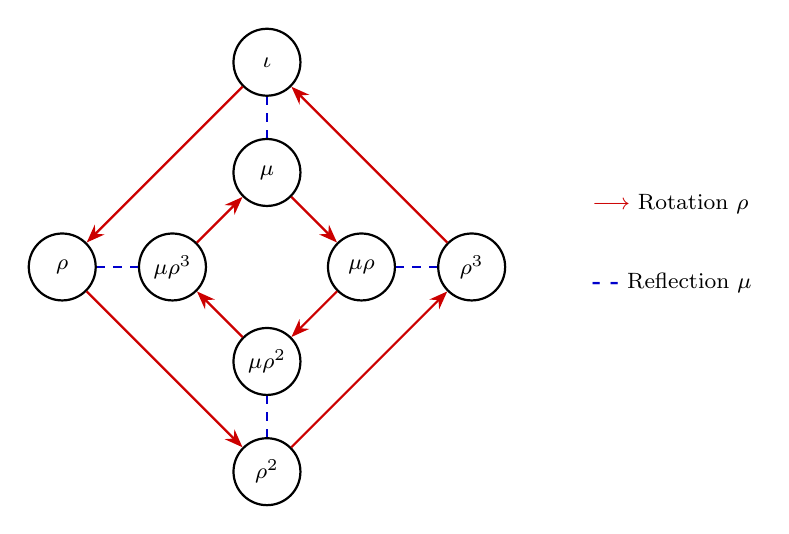
\begin{tikzpicture}[
        >=Stealth,
        thick,
        vtx/.style={circle, draw=black, fill=white, inner sep=1.5pt, minimum size=8.5mm, font=\footnotesize}
    ]
        % Outer Square: <rho>
        \node[vtx] (e)  at (90:2.6cm)  {$\iota$};
        \node[vtx] (r)  at (180:2.6cm) {$\rho$};
        \node[vtx] (r2) at (270:2.6cm) {$\rho^2$};
        \node[vtx] (r3) at (0:2.6cm)   {$\rho^3$};
    
        % Inner Square: mu<rho>
        \node[vtx] (m)   at (90:1.2cm)  {$\mu$};
        \node[vtx] (mr3) at (180:1.2cm) {$\mu\rho^3$};
        \node[vtx] (mr2) at (270:1.2cm) {$\mu\rho^2$};
        \node[vtx] (mr)  at (0:1.2cm)   {$\mu\rho$};
    
        % Outer cycle (solid red, counterclockwise)
        \draw[->, red!80!black] (e)  -- (r);
        \draw[->, red!80!black] (r)  -- (r2);
        \draw[->, red!80!black] (r2) -- (r3);
        \draw[->, red!80!black] (r3) -- (e);
    
        % Inner cycle (solid red, clockwise due to conjugation)
        \draw[->, red!80!black] (m)   -- (mr);
        \draw[->, red!80!black] (mr)  -- (mr2);
        \draw[->, red!80!black] (mr2) -- (mr3);
        \draw[->, red!80!black] (mr3) -- (m);
    
        % Radial reflections (dashed blue)
        \draw[blue!80!black, dashed] (e)  -- (m);
        \draw[blue!80!black, dashed] (r)  -- (mr3);
        \draw[blue!80!black, dashed] (r2) -- (mr2);
        \draw[blue!80!black, dashed] (r3) -- (mr);
    
        % Legend
        \node[anchor=west, font=\footnotesize] at (4.0, 0.8) {\textcolor{red!80!black}{$\longrightarrow$} Rotation $\rho$};
        \node[anchor=west, font=\footnotesize] at (4.0, -0.2) {\textcolor{blue!80!black}{\textbf{- -}} Reflection $\mu$};
    \end{tikzpicture}
    \end{figure}
    \bigskip

    \begin{ex}
        Let $G$ be an arbitrary group and let $a,b\in G$.
        \begin{itemize}
            \item Prove that if $\abs{ab}=n<\infty$, then $\abs{ba}=n$.
            \begin{proof}
                Notice
                \[
                    (ab)^n=a(ba)^{n-1}b=e\implies a(ba)^{n}=ea=a\implies (ba)^{n}=e\implies \abs{ba}\leq n
                \]
                and
                \[
                    ((ba)^m=e\implies (ab)^m=e)\implies \abs{ba}\geq\abs{ab}=n
                \]
                Then $\abs{ba}=n$.
            \end{proof}
            \item Deduce that for any $g\in G$ and $x\in G$, $\abs{x}=\abs{gxg^{-1}}$
            \begin{proof}
                We have
                \[
                    (gxg^{-1})^m=gx^mg^{-1}=e\implies gx^m=g\implies x^m=e\implies \abs{gxg^{-1}}\geq\abs{x}
                \]
                We also have
                \[
                    x^m=e\implies gx^mg^{-1}=e\implies gxg^{-1})^m=e\implies \abs{x}\geq\abs{gxg^{-1}}
                \]
                Therefore, $\abs{x}=\abs{gxg^{-1}}$.
            \end{proof}
            \begin{remark}
                In fact, let $a=gx$ and $b=g^{-1}$ then $\abs{ab}=\abs{gxg^{-1}}=\abs{ba}=\abs{x}$.
            \end{remark}
        \end{itemize}
    \end{ex}
    \bigskip

    \begin{ex}
        Let $H$ and $K$ be subgroups of a group $G$, and define the subset $HK=\set{hk:h\in H,k\in K}$
        \begin{itemize}
            \item Prove that if $G$ is abelian, then $HK\leq G$.
            \begin{proof}
                Let $hk,h'k'\in HK$, then we have
                \[
                    (hk)(h'k')^{-1}=hkk'^{-1}h'^{-1}=(hh'^{-1})(kk'^{-1})\in HK
                \]
                implying that $HK\leq G$.
            \end{proof}
            \item Give a counterexample when $G$ is nonabelian.
            \begin{proof}
                Let $G=D_3,H=\group{\mu},K=\group{\mu\rho}$, then $HK=\set{e,\mu,\rho,\mu\rho}$ is not a subgroup of $G$.
            \end{proof}
        \end{itemize}
    \end{ex}
    \bigskip

    \begin{ex}
        Let $G$ be a finite cyclic group. Prove that if $H,K\leq G$ with $H\noteq K$, then $\abs{H}\noteq\abs{K}$.
    \end{ex}
    \begin{proof}
        Let $G=\group{a}$ and $\abs{G}=n$. Then $H,K\leq G$ implies $H=\group{a^p}=\group{a^{\gcd(n,p)}},K=\group{a^q}=\group{a^{\gcd(n,q)}}$ for some $p,q\in\Z^+$, then 
        \[
            H\neq K\implies\gcd(n,p)\neq\gcd(n,q)\implies\abs{H}=\frac{n}{\gcd(n,p)}\neq\frac{n}{\gcd(n,q)}=\abs{K}
        \]
    \end{proof}
    \bigskip

    \begin{ex}
        Prove that a group $G$ with $\abs{G}>1$ has no proper nontrivial subgroups if and only if $G$ is finite and is isomorphic to $\Z_p$ for some prime $p$.
    \end{ex}
    \begin{proof}
        $\implies:$ Let $a\neq e\in G$.. Then $\group{a}\leq G$ must equals $G$ for otherwise it will be a proper nontrivial subgroup of $G$. Then $G$ is cyclic. If $G$ is infinite, then $\group{a}=\group{a^2}=G$ leads to a contradiction since $a\notin\group{a^2}$. If $\abs{G}=mn$ for some $m,n>1$, then $\abs{a^m}=mn/\gcd(mn,m)=n$ implying that $\group{a^m}$ is a proper nontrivial subgroup of $G$. Therefore, $G=\group{a}$ and $\abs{G}=p$ with $p$ prime. It follows that $G\cong\Z_p$.

        $\impliedby:$ Let $G\cong\Z_p$, then $G=\group{a}$ and $\abs{G}=p$. If $H\leq G$, then $H=\group{a^s}=\group{a^{\gcd(p,s)}}$. Since $p$ is prime, we know $H=\set{e}$ or $H=G$.
    \end{proof}
    
    \subsection{Finitely Generated Abelian Groups}
    
    \begin{defi}{Direct Product of Groups}
        Let $G_1, G_2, \ldots, G_n$ be groups. The \textbf{direct product} $\prod_{i=1}^n G_i = G_1 \times G_2 \times \cdots \times G_n$ is the Cartesian product endowed with componentwise binary operation:
        \[
            (a_1, a_2, \ldots, a_n)(b_1, b_2, \ldots, b_n) = (a_1 b_1, a_2 b_2, \ldots, a_n b_n).
        \]
        The identity element is $(e_1, e_2, \ldots, e_n)$, and $(a_1, \ldots, a_n)^{-1} = (a_1^{-1}, \ldots, a_n^{-1})$. It therefore forms a group.
    \end{defi}
    \bigskip

    \begin{thm}\label{0.2.2}
        The group $\prod_{i=1}^n \Z_{m_i}$ is cyclic and isomorphic to $\Z_{m_1 m_2 \cdots m_n}$ if and only if $\gcd(m_i, m_j) = 1$ for all $i \noteq j$.
    \end{thm}
    \bigskip

    \begin{thm}
        Let $(a_1, a_2, \ldots, a_n) \in \prod_{i=1}^n G_i$. If each $a_i$ has finite order $r_i$ in $G_i$, then
        \[
            \abs{(a_1, a_2, \ldots, a_n)} = \lcm(r_1, r_2, \ldots, r_n).
        \]
    \end{thm}
    \bigskip

    \begin{thm}[\textbf{Fundamental Theorem of Finitely Generated Abelian Groups - Primary Factor Form}]
        Every finitely generated abelian group $G$ is isomorphic to a direct product of cyclic groups:
        \[
            G \cong \Z_{(p_1)^{r_1}} \times \Z_{(p_2)^{r_2}} \times \cdots \times \Z_{(p_n)^{r_n}} \times \underbrace{\Z \times \cdots \times \Z}_{\beta \text{ copies}},
        \]
        where $p_i$ are primes (not necessarily distinct) and $r_i \in \Z^+$. $\beta$ is called the \textbf{Betti number} of $G$.
    \end{thm}
    \bigskip

    \begin{thm}[\textbf{Fundamental Theorem of Finitely Generated Abelian Groups - Invariant Factor Form}]
        Every finitely generated abelian group $G$ is isomorphic to a direct product of cyclic groups:
        \[
            G \cong \Z_{d_1} \times \Z_{d_2} \times \cdots \times \Z_{d_k} \times \underbrace{\Z \times \cdots \times \Z}_{\beta \text{ copies}},
        \]
        where each $d_i \ge 2$ and $d_1 \mid d_2 \mid \cdots \mid d_k$. The \textbf{invariant factors} $d_1, \ldots, d_k$ and the Betti number $\beta$ are uniquely determined.
    \end{thm}
    \bigskip

    \begin{defi}{Decomposable and Indecomposable Groups}
        A group $G$ is \textbf{decomposable} if it is isomorphic to the direct product of two proper nontrivial subgroups: $G \cong H \times K$ with $H, K \noteq \set{e}$. Otherwise, $G$ is \textbf{indecomposable}.
    \end{defi}
    \bigskip

    \begin{thm}
        \[
            G \text{ is finite indecomposable abelian} \iff G \cong \Z_{p^r} \text{ for some prime } p \text{ and } r \in \Z^+.
        \]
    \end{thm}
    \bigskip

    \begin{thm}
        If $G$ is a finite abelian group and $m \mid \abs{G}$, then $G$ contains a subgroup of order $m$.
    \end{thm}
    \bigskip

    \begin{thm}
        If $m \in \Z^+$ is square-free, then every abelian group of order $m$ is cyclic.
    \end{thm}
    \bigskip
    
    \begin{ex}
        Let $G=\Z_4\times\Z_{18}\times\Z_{15}$ and $H=\Z_3\times\Z_{36}\times\Z_{10}$. Are they isomorphic?
    \end{ex}
    \begin{proof}
        We have 
        \[
            G\cong\Z_4\times(\Z_2\times\Z_9)\times(\Z_3\times\Z_5)
        \]
        and 
        \[
            H\cong\Z_3\times(\Z_4\times\Z_9)\times(\Z_2\times\Z_5)
        \]
        It follows that $G\cong H$.
    \end{proof}
    \bigskip

    \begin{ex}
        Let $G$ be a finite abelian group. Prove that $G$ is not cyclic if and only if $G$ contains a subgroup isomorphic to $\Z_p\times\Z_p$ for some prime $p$.
    \end{ex}
    \begin{proof}
        Since $G$ is finite abelian, then
        \[
            G\cong\prod_{i=1}^n\Z_{(p_i)^{r_i}}
        \]
        By \hyperref[0.2.2]{Theorem 0.2.2}, if it is not cyclic, then $\gcd((p_i)^{r_i},(p_j)^{r_j})>1$ for some $i\neq j$, implying that $p_i=p_j$ and then
        \[
            \Z_{p_i}\times\Z_{p_i}\cong\group{(p_i)^{r_i-1}}\times\group{(p_j)^{r_j-1}}\leq\Z_{(p_i)^{r_i}}\times\Z_{(p_j)^{r_j}}\leq\prod_{i=1}^n\Z_{(p_i)^{r_i}}\cong G
        \]
        If $G$ is cylic, then $p_i\neq p_j$ for all $i\neq j$. It follows that if $H\leq G$, then
        \[
            H\cong\prod_{i=1}^nZ_{(p_i)^{q_i}},q_i\leq r_i
        \]
        which is not isomorphic to $\Z_p\times\Z_p$ since $p_i$ are mutually distinct.
    \end{proof}
    \begin{remark}
        In fact, when $G$ is cylic, we can deduce that $H\leq G$ is also cyclic, which directly tells proves the result.
    \end{remark}
    \begin{remark}
        Generally, one can prove that:
        \begin{quote}
            Let $G$ be a finite abelian group, and let $x_1,\dots,x_n\geq 2$ be integers. The group $H=\prod_{i=1}^n\Z_{x_i}$ is isomorphic to a subgroup of $G$ if and only if $G$ can be decomposed as a direct product of cyclic groups $G\cong\prod_{j=1}^m\Z_{y_j}$ such that $m\geq n$ and $x_i\mid y_i$ for all $i\in\set{1,\dots,n}$.
        \end{quote}
    \end{remark}
    \hfill

    \begin{ex}
        Let $G,H,K$ be finitely generated abelian groups. Show that
        \[
            G\times K\cong H\times K\implies G\cong H
        \]
    \end{ex}
    \begin{proof}
        Since $G,H,K$ are finitely generated abelian groups, so are $G\times K$ and $H\times K$. Since $G\times K\cong H\times K$, so they have the same Betti number and the same collection of $(p_i)^{r_i}$ after decomposition. It follows that after picking up the part given by $K$, we know $G$ and $H$ have the same Betti number and the same collection of $(p_i)^{r_i}$ after decomposition, which implies $G\cong H$.
    \end{proof}

    \subsection{Cosets and the Theorem of Lagrange}

    \begin{thm}
        Let $H \le G$. The relation $\sim_L$ defined on $G$ by
        \[
            a \sim_L b \iff a^{-1}b \in H
        \]
        is an equivalence relation on $G$. Similarly, $a \sim_R b \iff ab^{-1} \in H$ is an equivalence relation.
    \end{thm}
    \bigskip

    \begin{defi}{Coset}
        Let $H \le G$ and $a \in G$.
        \begin{itemize}
            \item The \textbf{left coset} of $H$ containing $a$ is the equivalence class under $\sim_L$:
            \[
                aH = \set{ah \mid h \in H}.
            \]
            \item The \textbf{right coset} of $H$ containing $a$ is the equivalence class under $\sim_R$:
            \[
                Ha = \set{ha \mid h \in H}.
            \]
        \end{itemize}
    \end{defi}
    \bigskip

    \begin{thm}
        Let $H \le G$. For every $a \in G$, the map $f \colon H \to aH$ defined by $f(h) = ah$ is a bijection. Consequently,
        \[
            \abs{aH} = \abs{H} = \abs{Ha} \quad (\forall a \in G).
        \]
    \end{thm}
    \bigskip

    \begin{thm}[Theorem of Lagrange]
        Let $H$ be a subgroup of a finite group $G$. Then the order of $H$ divides the order of $G$:
        \[
            \abs{H} \mid \abs{G}.
        \]
    \end{thm}
    
    \begin{cor}\label{0.3.5}
        Every group of prime order $p$ is cyclic, hence isomorphic to $\Z_p$.
    \end{cor}
    \bigskip

    \begin{thm}
        Let $G$ be a finite group. For every $g \in G$, $\abs{g}$ divides $\abs{G}$. In particular, $g^{\abs{G}} = e$.
    \end{thm}
    \bigskip

    \begin{defi}{Index of a Subgroup}
        Let $H \le G$. The \textbf{index} of $H$ in $G$, denoted $(G : H)$ or $[G : H]$, is the cardinality of the set of left (or right) cosets of $H$ in $G$. When $G$ is finite,
        \[
            [G : H] = \frac{\abs{G}}{\abs{H}}.
        \]
    \end{defi}
    \bigskip

    \begin{thm}[Tower Law for Subgroup Indices]
        Let $K \le H \le G$. If $[G : H]$ and $[H : K]$ are finite, then $[G : K]$ is finite and
        \[
            [G : K] = [G : H] \cdot [H : K].
        \]
    \end{thm}
    \bigskip

    \begin{thm}[Cosets of Homomorphism Kernels]
        Let $\phi \colon G \to G'$ be a group homomorphism. Then
        \begin{enumerate}
            \item Left and right cosets of $\ker(\phi)$ coincide:
            \[
                a \ker(\phi) = \ker(\phi) a \quad (\forall a \in G).
            \]
            \item Two elements $a, b \in G$ belong to the same coset of $\ker(\phi)$ if and only if $\phi(a) = \phi(b)$:
            \[
                a \ker(\phi) = b \ker(\phi) \iff \phi(a) = \phi(b).
            \]
        \end{enumerate}
    \end{thm}
    \bigskip

    \begin{cor}
        A group homomorphism $\phi \colon G \to G'$ is injective if and only if
        \[
            \ker(\phi) = \set{e_G}.
        \]
    \end{cor}
    \bigskip

    \begin{ex}
        Let $\sigma=(1,2,5,4)(2,3)$ in $S_5$, find the index of $\group{\sigma}$ in $S_5$.
    \end{ex}
    \begin{proof}
        Notice $\sigma=(1,2,3,5,4)$, then the order of $\sigma$ is $5$ in $S_5$, implying the index given by 
        \[
            [S_5:\group{\sigma}]=\frac{\abs{S_5}}{\abs{\group{\sigma}}}=\frac{5!}{5}=24
        \]
    \end{proof}
    \bigskip

    \begin{ex}
        Let $H$ be a subgroup of a group $G$, let $a,b\in G$. Is it true that 
        \[
            aH=bH\implies Ha^{-1}=Hb^{-1}
        \]
    \end{ex}
    \begin{proof}
        The statement is true. Since $aH=bH$, then $ah_a=bh_b$ for some $h_a,h_b\in H$, it follows that $b^{-1}a\in H$. Therefore, for $hb^{-1}\in Hb^{-1}$, we have $hb^{-1}=hb^{-1}aa^{-1}=(hb^{-1}a)a^{-1}\in Ha^{-1}$. Then $Hb^{-1}\subset Ha^{-1}$, similarly we can deduce that $H^{-1}\subset Hb^{-1}$, thus $Ha^{-1}=Hb^{-1}.$
    \end{proof}
    \bigskip

    \begin{ex}
        Let $G$ be a group of order $pq$, where $p$ and $q$ are prime numbers. Show that every proper subgroup of $G$ is cyclic.
    \end{ex}
    \begin{proof}
        By Theorem of Lagrange we know every proper subgroup $H$ has order $\abs{H}=n\mid pq$ implying $n=1$ or $n=p$ or $n=q$. If $n=1$ then $H$ is trivially cyclic, if $n=p$ or $n=q$ then \hyperref[0.3.5]{Corollary 0.3.5} tells that $H$ is cyclic.         
    \end{proof}


    % --- Back Matter ---
    \printglossary
    
\end{document}